%% line1.tex
\documentclass{standalone}
\usepackage{tkz-euclide}
\usetkzobj{all}
%% ================== commands ==========================
\newcommand{\myShowPoints}[2]{
\tkzDrawPoints(#1) 
\tkzLabelPoints[#2](#1)
}		
\newcommand{\myGetMidPoint}[3]{
\tkzDefMidPoint(#1,#2)\tkzGetPoint{#3}
}		
\begin{document}
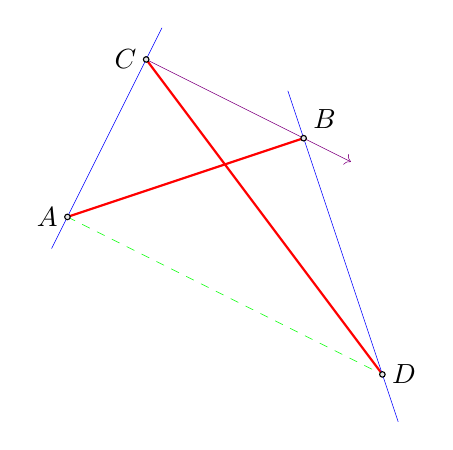
\begin{tikzpicture}
	\tkzDefPoint(-3,0){A}
	\tkzDefPoints{0/1/B, -2/2/C, 1/-2/D}
	% drawing red segments
	\tkzDrawSegments[red, thick](A,B C,D)
	% drawing dashed green segment
	\tkzDrawSegments[green,dashed](A,D)
	% drawing blue line
	\tkzDrawLines[draw =blue](A,C B,D)
	% array with arrow
	\tkzDrawLines[add = 0 and 0.3, draw=violet, arrows=->](C,B)
	% show points
	\myShowPoints{A,C}{left}
	\myShowPoints{D}{right}
	\myShowPoints{B}{above right}
\end{tikzpicture}
\end{document}